\documentclass[12pt,letterpaper]{article}
\usepackage{fullpage}
\usepackage[top=2cm, bottom=4.5cm, left=2.5cm, right=2.5cm]{geometry}
\usepackage{amsmath,amsthm,amsfonts,amssymb,amscd}
\usepackage{lastpage}
\usepackage{enumerate}
\usepackage{fancyhdr}
\usepackage{mathrsfs}
\usepackage{xcolor}
\usepackage{graphicx}
\usepackage{listings}
\usepackage{hyperref}

\hypersetup{%
  colorlinks=true,
  linkcolor=blue,
  linkbordercolor={0 0 1}
}
 
\renewcommand\lstlistingname{Algorithm}
\renewcommand\lstlistlistingname{Algorithms}
\def\lstlistingautorefname{Alg.}

\lstdefinestyle{Python}{
    language        = Python,
    frame           = lines, 
    basicstyle      = \footnotesize,
    keywordstyle    = \color{blue},
    stringstyle     = \color{green},
    commentstyle    = \color{red}\ttfamily
}

\setlength{\parindent}{0.0in}
\setlength{\parskip}{0.05in}

% Edit these as appropriate
\newcommand\course{CSE 3500}
\newcommand\hwnumber{1}                  % <-- homework number
\newcommand\NetIDa{netid19823}           % <-- NetID of person #1
\newcommand\NetIDb{netid12038}           % <-- NetID of person #2 (Comment this line out for problem sets)

\pagestyle{fancyplain}
\headheight 35pt
\lhead{\NetIDa}
\lhead{\NetIDa\\\NetIDb}                 % <-- Comment this line out for problem sets (make sure you are person #1)
\chead{\textbf{\Large Homework \hwnumber}}
\rhead{\course \\ \today}
\lfoot{}
\cfoot{}
\rfoot{\small\thepage}
\headsep 1.5em

\begin{document}

\section*{Problem 1}

Answer to the problem goes here.

\begin{enumerate}
  \item
   Problem 1 part 1 answer here.
  \item
    Problem 1 part 2 answer here.

    Here is an example typesetting mathematics in \LaTeX
\begin{equation*}
    X(m,n) = \left\{\begin{array}{lr}
        x(n), & \text{for } 0\leq n\leq 1\\
        \frac{x(n-1)}{2}, & \text{for } 0\leq n\leq 1\\
        \log_2 \left\lceil n \right\rceil \qquad & \text{for } 0\leq n\leq 1
        \end{array}\right\} = xy
\end{equation*}

    \item Problem 1 part 3 answer here.

    Here is an example of how you can typeset algorithms.
    There are many packages to do this in \LaTeX.
     
    \lstset{caption={Caption for code}}
    \lstset{label={lst:alg1}}
     \begin{lstlisting}[style = Python]
    from package import Class # Mesh required for..
    
    cinstance = Class.from_obj('class.obj')
    cinstance.go()
    \end{lstlisting}
     
  \item Problem 1 part 4 answer here.

    Here is an example of how you can insert a figure.
    \begin{figure}[!h]
    \centering
    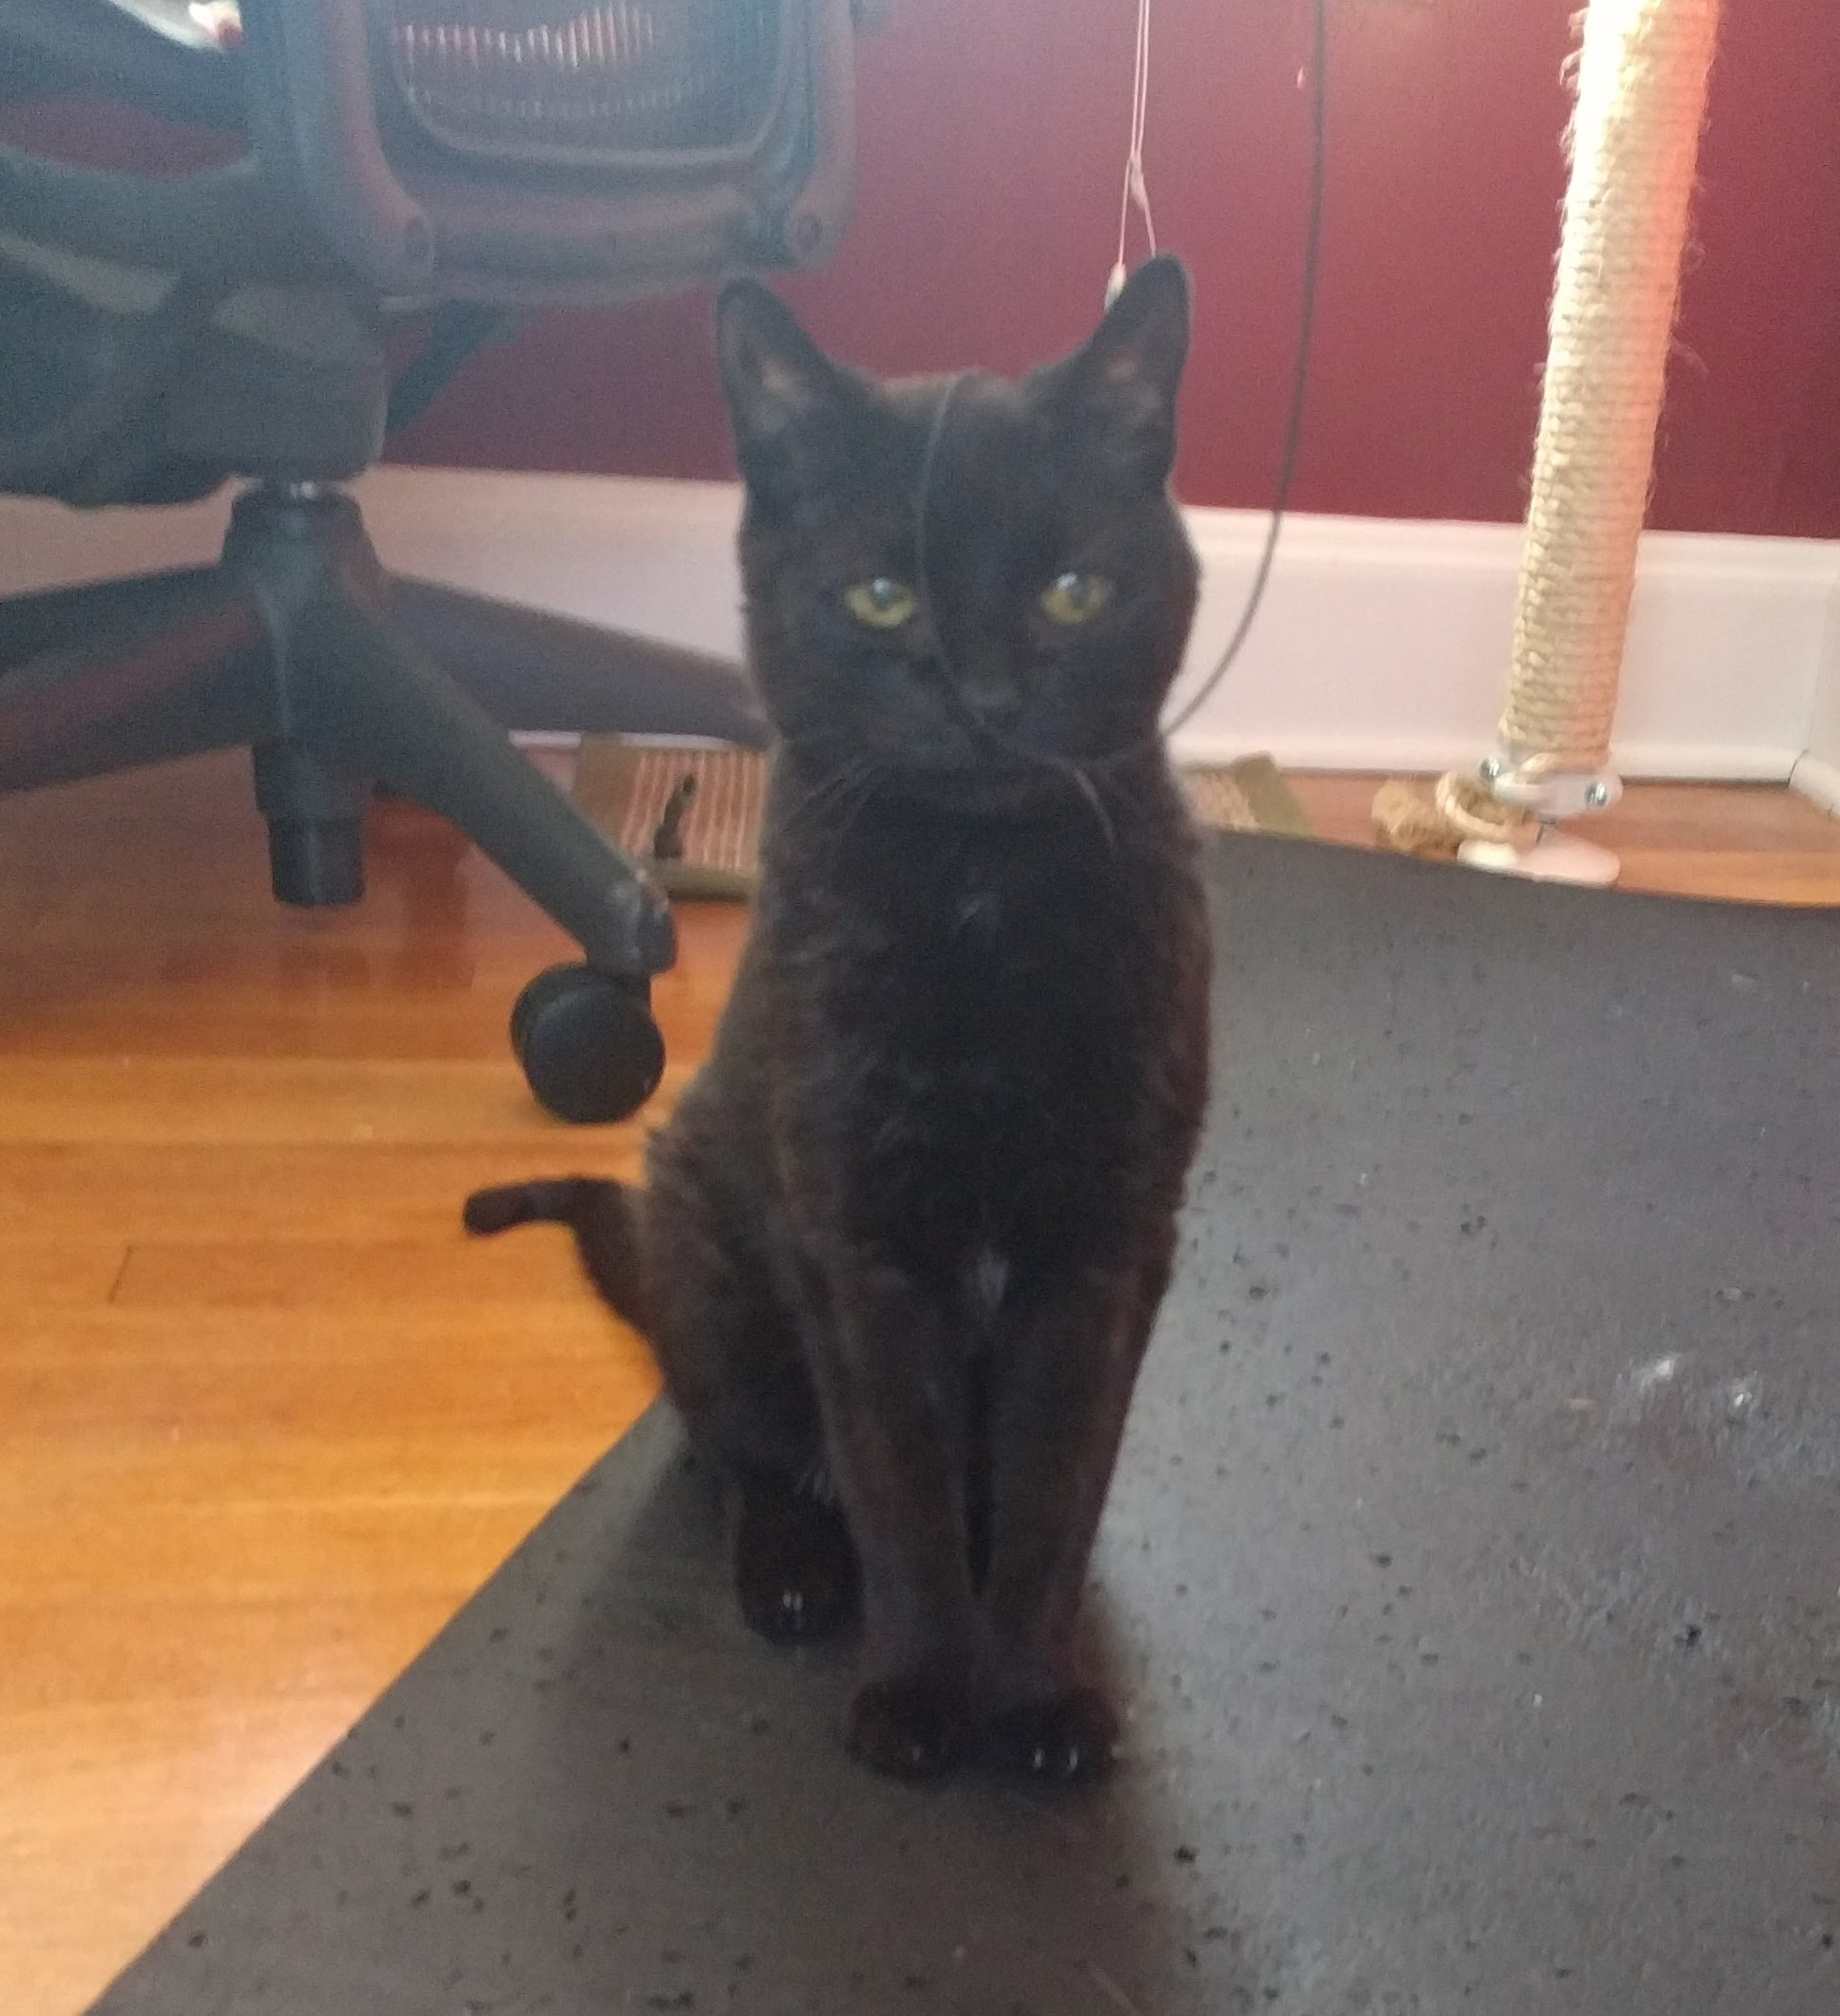
\includegraphics[width=0.3\linewidth]{heidi.jpg}
    \caption{Heidi attacked by a string.}
    \end{figure}
\end{enumerate}


\section*{Problem 2}
% Rest of the work...

\end{document}
